\documentclass[main.tex]{subfiles}

\begin{document}
\section{整体设计}
\subsection{CPU整体框图}
CPU整体设计如下方框图所示。图中白色方框为模块,浅橙色梯形为MUX,紫色方框为32位寄存器,箭头连线为数据连接线,彩色图形为控制信号。
\begin{figure}[h]
\centering
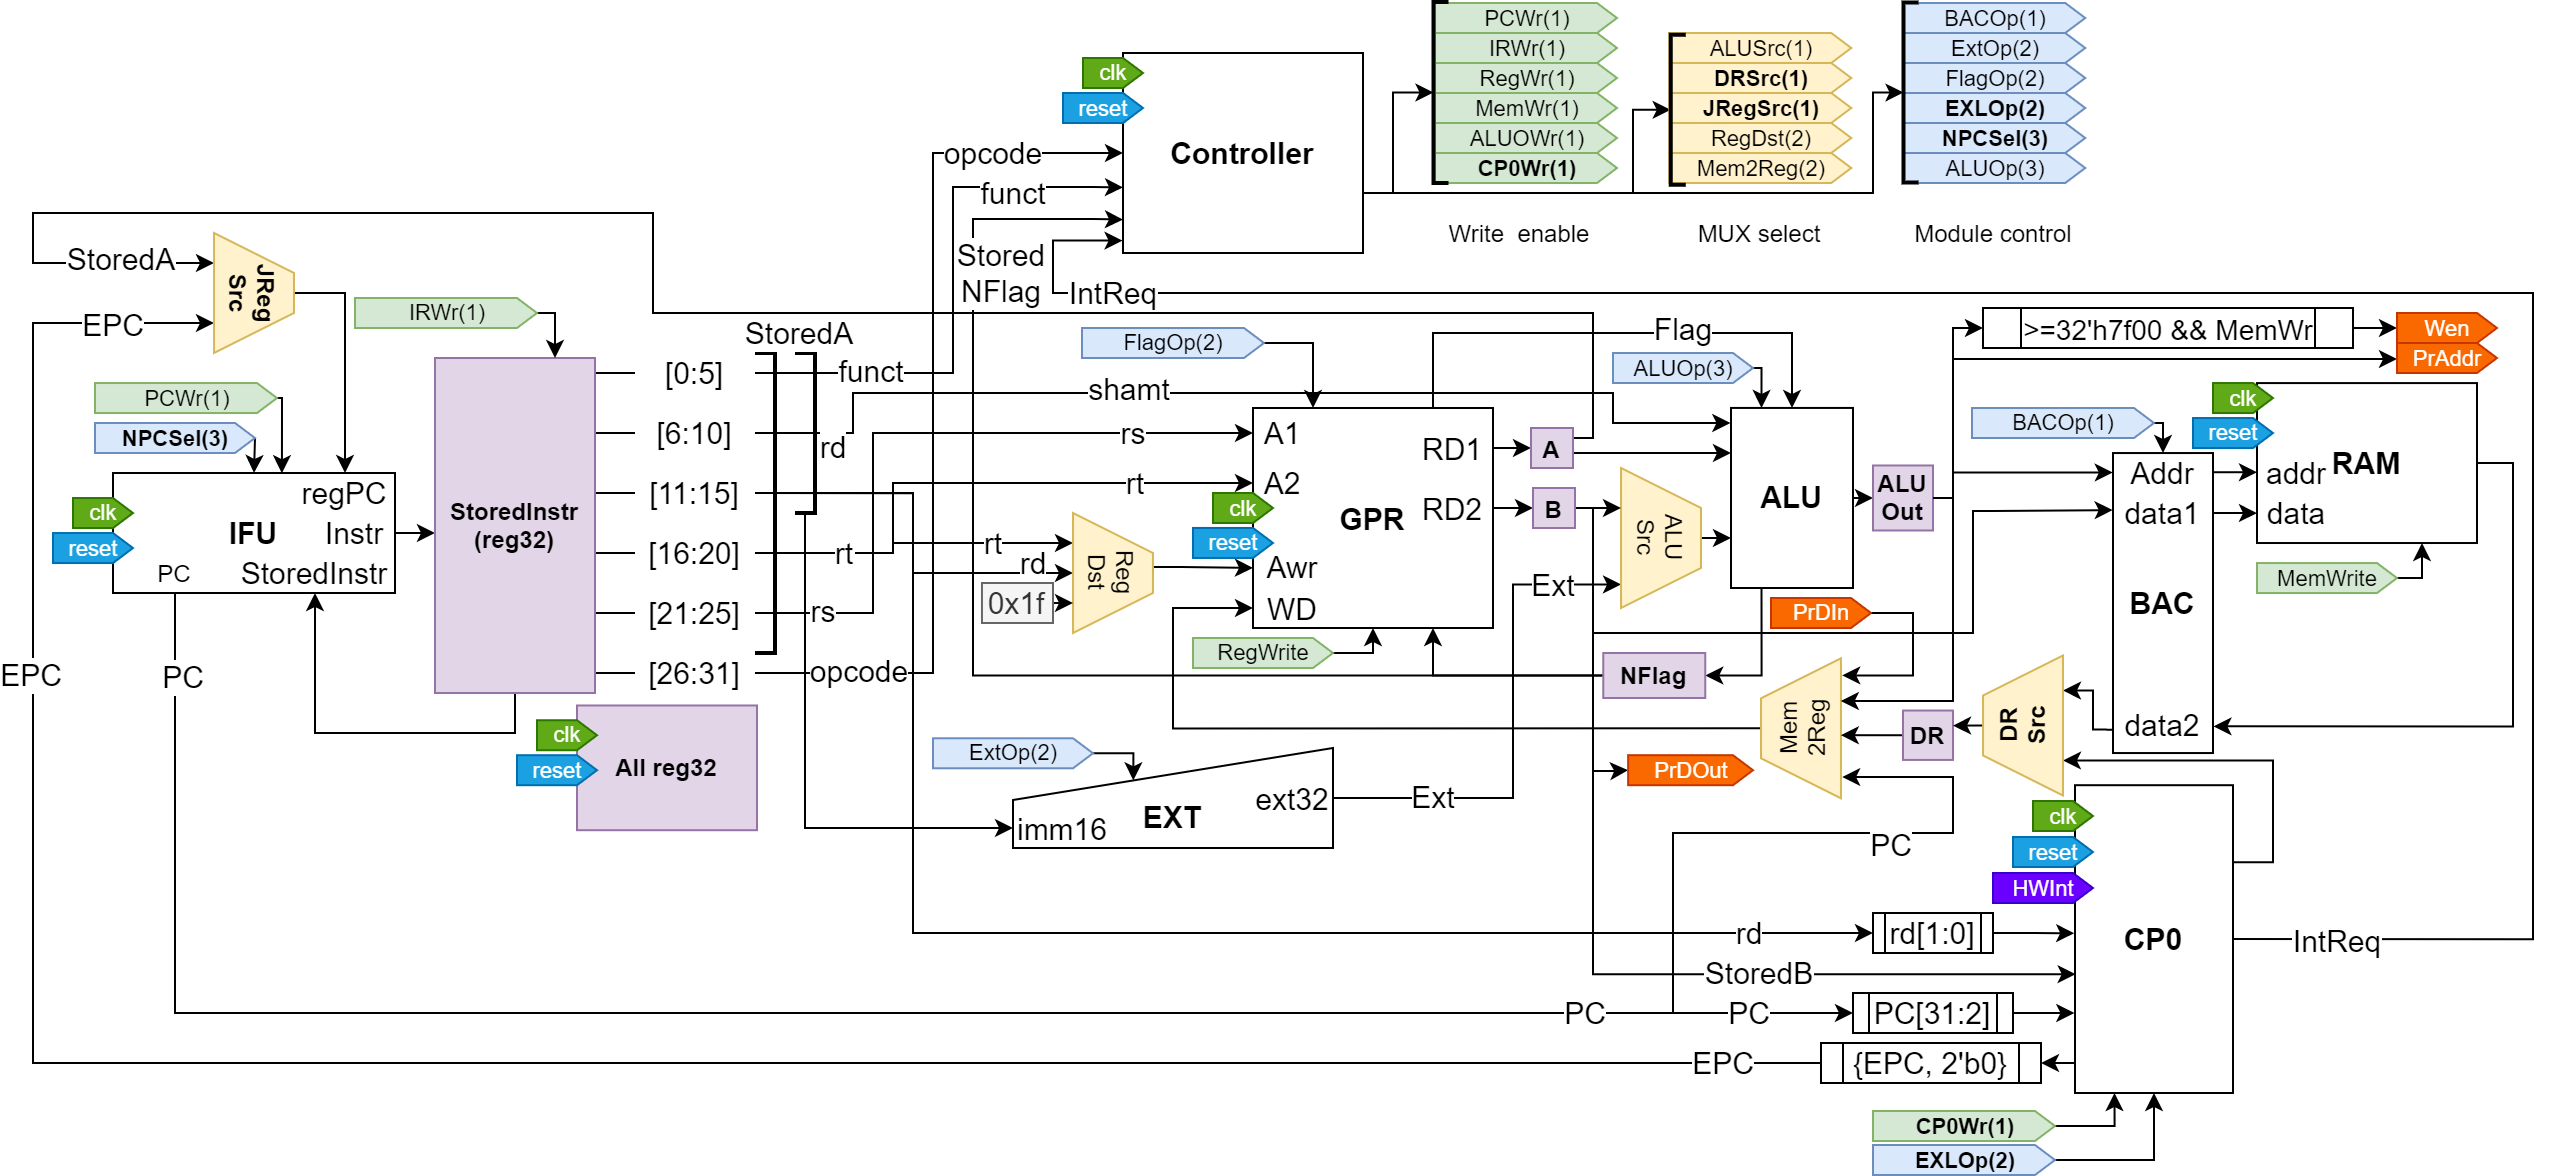
\includegraphics[width=\textwidth]{images/PCOCD-P3-mips-block.png}
\caption{CPU整体框图}
\end{figure}

图中共有$7$个模块,分别与任务要求的七个模块对应,实现的功能与课程要求一致。

图中共有$17$路控制信号,均由$Controller$模块产生。具体功能见下表。

\begin{center}
    \captionof{table}{控制信号说明}
    \begin{tabular}{c c c c c}
        \toprule
        标识颜色 & 控制信号类型 & 位宽 & 作用元件 & 效果\\
        \midrule
         绿色 & 写入使能信号 & 1bit & 存储器(寄存器组、内存) & 高有效写入使能 \\
         黄色 & 数据控制信号 & 1-2bit & 32bit二选一MUX & 从两至三路信号中选择一路 \\
         蓝色 & 模块功能信号 & 2-3bit & 多功能模块 & 选择模块功能 \\
        \bottomrule
    \end{tabular}
\end{center}

图中共有$7$路外部输入信号:时钟信号$clk$和系统重置信号$reset$,硬件中断信号$HWInt$,与$Bridge$交互的四路信号$PrDIn$、$PrAddr$、$PrDOut$和$Wen$。

\clearpage

\begin{figure}[h]
  \begin{adjustbox}{addcode={\begin{minipage}{\width}}{\caption{Project3 CPU模块mips框图}\end{minipage}},rotate=90,center}
		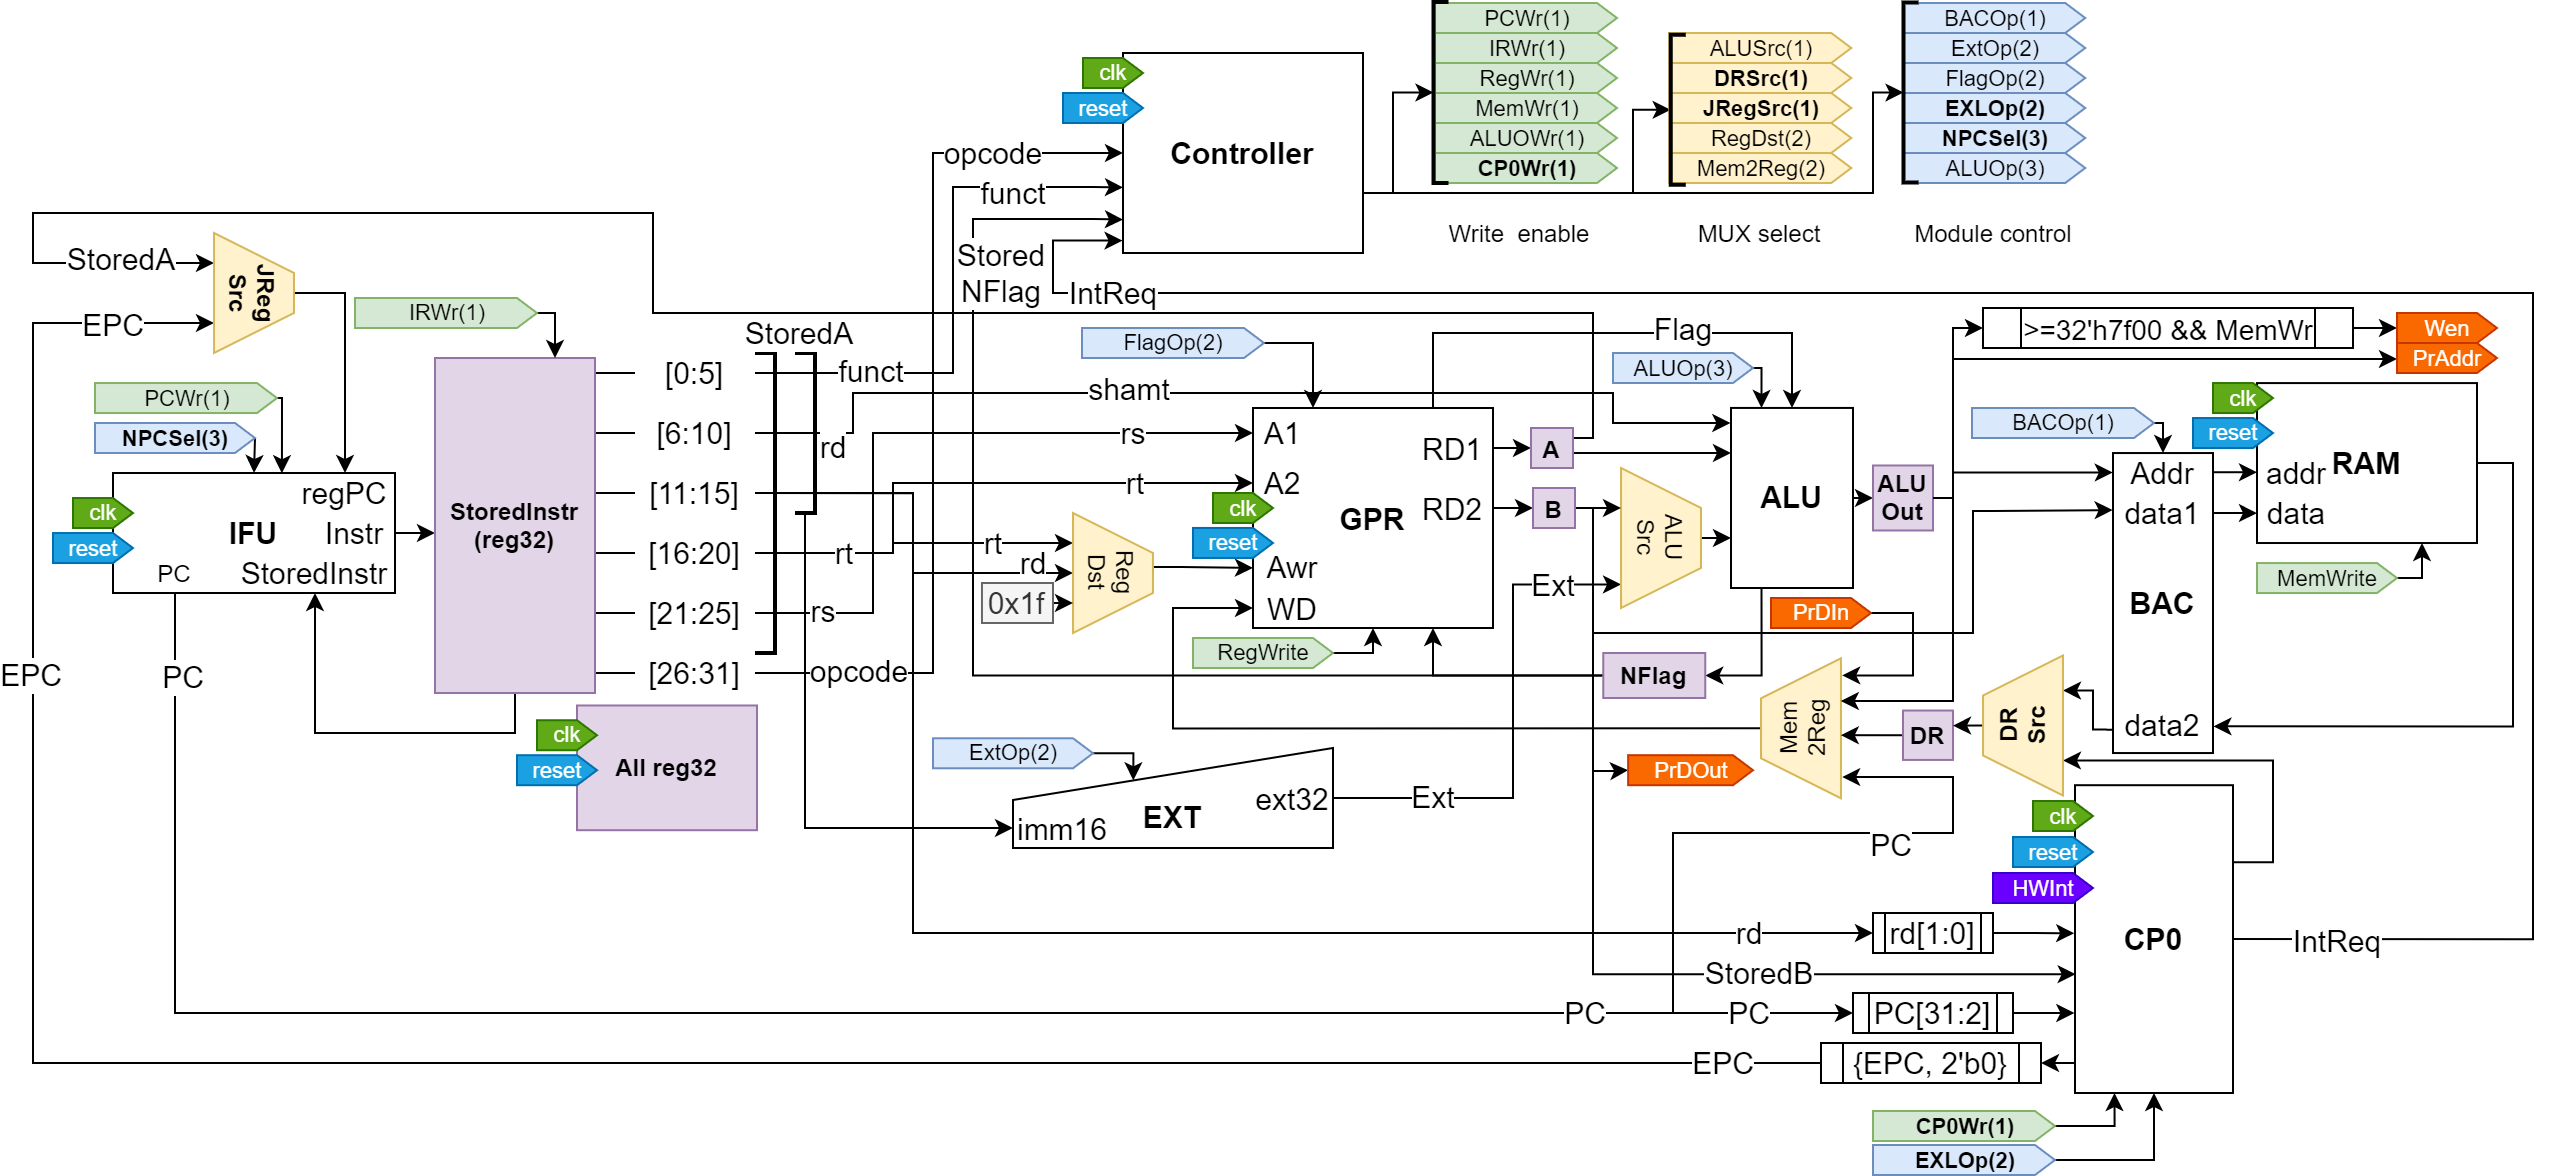
\includegraphics[width=10 in]{images/PCOCD-P3-mips-block.png}%
	\end{adjustbox}
\end{figure}
\clearpage

\subsection{系统整体框图}
系统整体设计如下方框图所示。
\begin{figure}[h]
\centering
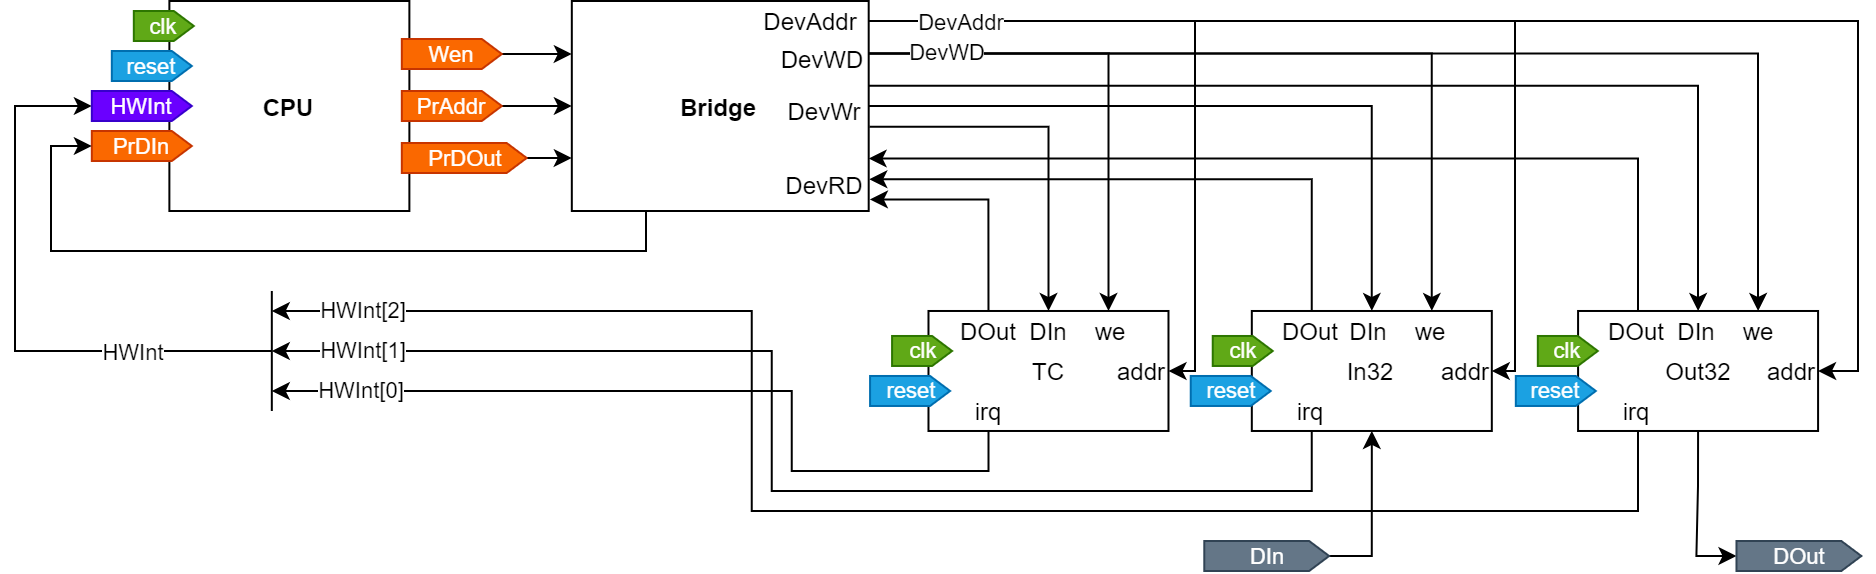
\includegraphics[width=\textwidth]{images/PCOCD-P3-main-block.png}
\caption{系统整体框图}
\end{figure}

图中CPU为上一页中的CPU整体。其余的模块为三个外设以及使得它们与CPU连通的$Bridge$。

图中共有四路外部输入信号:时钟信号$clk$和系统重置信号$reset$,数据输入输出$DIn$和$DOut$。

\clearpage

\begin{figure}[h]
  \begin{adjustbox}{addcode={\begin{minipage}{\width}}{\caption{Project3 顶层模块main框图}\end{minipage}},rotate=90,center}
		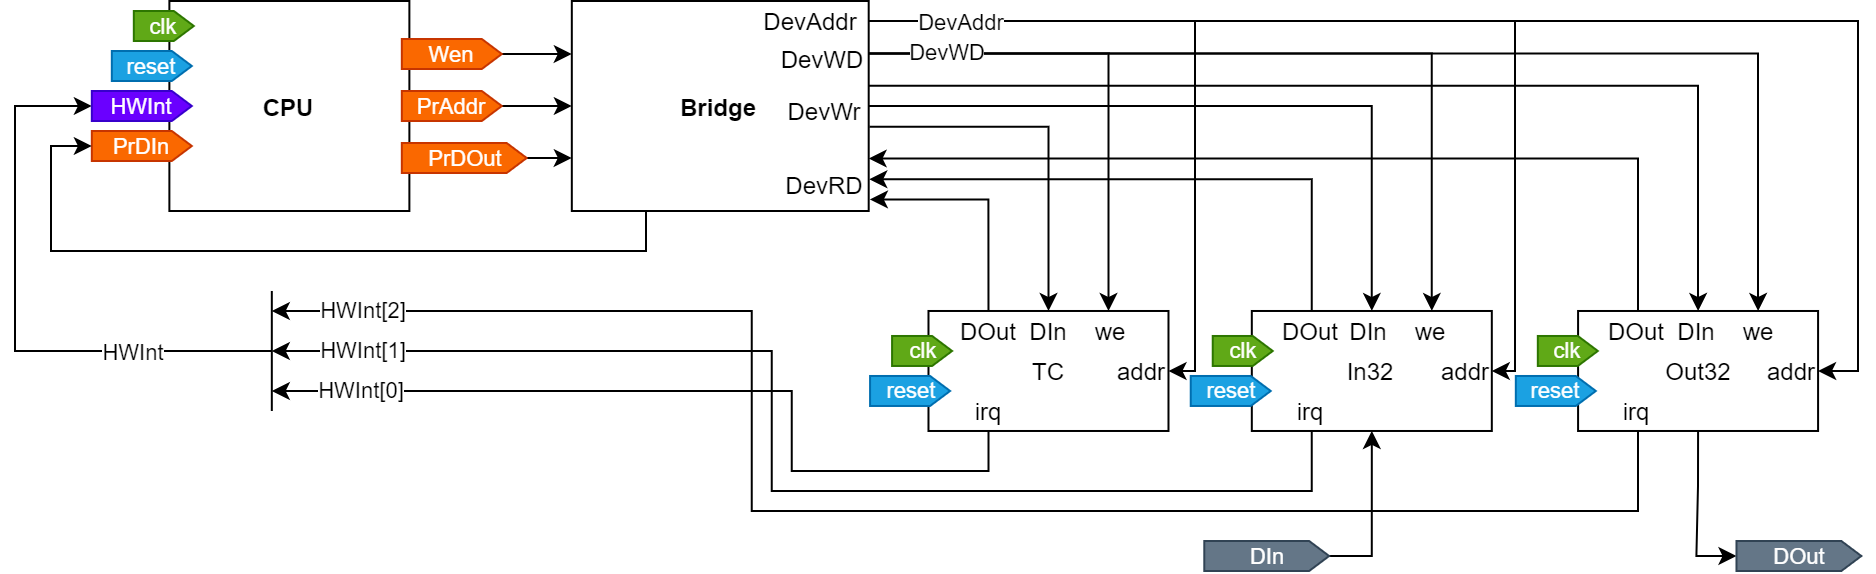
\includegraphics[width=10 in]{images/PCOCD-P3-main-block.png}%
	\end{adjustbox}
\end{figure}
\clearpage

\end{document}
